\chapter*{ECRICOME 2017 : le sujet}
  
%

\section*{Exercice 1}

\noindent
Dans tout l'exercice, on notera $\M{3}$ l'ensemble des matrices
carrées d'ordre $3$ et $I$ la matrice identité d'ordre $3$. On
considère la matrice $a$ définie par :
\[
A = 
\begin{smatrix}
  0 & 1 & 2\\
  -1 & 2 & 2\\
  -3 & 3 & 1
\end{smatrix}
\]

\subsection*{Partie A : Étude de la matrice $A$}
\begin{noliste}{1.}
\item Calculer les matrices $(A-I)^2$ et $(A-I)^3$.



\item En déduire l'ensemble des valeurs propres de $A$.



\item La matrice $A$ est-elle inversible ? Est-elle diagonalisable ?

  
\end{noliste}


%\newpage


\subsection*{Partie B : Recherche d'une solution particulière}
\noindent
On note pour tout $x\in \ ]-1,1[$, $\varphi(x)=\sqrt{1+x}$.
\begin{noliste}{1.}
  \setcounter{enumi}{3}
\item Justifier que la fonction $\varphi$ est de classe $\Cont 2$ sur 
  $]-1,1[$, et déterminer les valeurs de $\varphi'(0)$ et $\varphi''(0)$.
  
  

\item En utilisant la formule de Taylor-Young pour $\varphi$ en $0$ à
  l'ordre $2$, déterminer un réel $\alpha$ non nul tel que :
  \[
  \sqrt{1+x} = 1 + \frac{1}{2}x + \alpha x^2 + x^2 \varepsilon(x)
  \qquad \mbox{ avec } \quad \dlim{x\to 0} \varepsilon(x) = 0.
  \]
  
  

\item On note $P(x)=1+\frac{1}{2}x+\alpha x^2$ la fonction polynomiale
  de degré $2$ ainsi obtenue. Développer $(P(x))^2$.
  
  
  
  
  %\newpage
  
  
\item Soit $C=A-I$. En utilisant les résultats de la question
  \itbf{1.}, vérifier que $\big(P(C)\big)^2 = A$.\\
  Expliciter alors une matrice $M$ telle que $M^2=A$.
  
  
\end{noliste}

\subsection*{Partie C : Résolution complète de l'équation}
\noindent
On munit l'espace vectoriel $\R^3$ de sa base canonique 
$\B=(e_1,e_2,e_3)$.\\
Soit $f$ l'endomorphisme de $\R^3$ dont la matrice représentative dans 
la base $\B$ est la matrice $A$.\\
Dans cette partie, on pose : $T=\begin{smatrix}
  1 & 1 & 0\\ 0 & 1 & 1\\ 0 & 0 & 1
\end{smatrix}$.
\begin{noliste}{1.}
  \setcounter{enumi}{7}
\item Soient $u$, $v$ et $w$ les vecteurs définis par : $\left\{ 
    \begin{array}{l}
      w=(1,0,1),\\
      v=f(w)-w,\\
      u=f(v)-v.
    \end{array}\right.$
  \begin{noliste}{a)}
  \item Calculer les vecteurs $v$ et $u$.
    
    
    
	
    %\newpage
	
	
  \item Démontrer que la famille $\B'=(u,v,w)$ est une base de $\R^3$.
    
    
    
  \item Déterminer la matrice représentative de $f$ dans la base
    $\B'$.
    
    
    
  \item En déduire qu'il existe une matrice $P\in\M{3}$ 
    inversible telle que $T=P^{-1}AP$.
    
    
  \end{noliste}
  
\item Soit $N\in\M{3}$.
  \begin{noliste}{a)}
  \item Montrer que si $N^2=T$, alors $NT=TN$. En déduire que $N$ 
    est de la forme :
    \[
    N=
    \begin{smatrix} 
      a & b & c\\ 
      0 & a & b\\ 
      0 & 0 & a
    \end{smatrix},
    \]
    où $a$, $b$ et $c$ sont trois réels.
    
    
    \newpage
    
    
  \item Démontrer alors que l'équation matricielle $N^2=T$ admet
    exactement $2$ solutions $N_1$ et $N_2$.
    
    
  \end{noliste}
  
\item Montrer que l'équation matricielle $M^2=A$ d'inconnue
  $M\in\M{3}$ admet exactement deux solutions que l'on écrira en
  fonction de $P$, $P^{-1}$, $N_1$ et $N_2$.

  
  
\item L'ensemble $E$ des matrices $M$ appartenant à $\M{3}$ telles que
  $M^2=A$ est-il un espace vectoriel ?

  
\end{noliste}




%\newpage




\section*{Exercice 2}
\noindent
Dans tout l'exercice, $a$ est un réel strictement positif.

\subsection*{Partie A}
\noindent
On considère la fonction $\varphi$ définie sur $\R_+^*$ par : $\forall 
x>0$, $\varphi(x)=\ln(x)-ax^{2a}$.
\begin{noliste}{1.}
\item Déterminer $\dlim{x\to 0} \varphi(x)$ et $\dlim{x\to+\infty}
  \varphi(x)$.

  
  
\item Étudier les variations de la fonction $\varphi$ et dresser son
  tableau de variations.\\
  On fera apparaître dans ce tableau le réel $x_0 =
  \left(\dfrac{1}{2a^2}\right)^{\frac{1}{2a}}$.

  
  
\item Démontrer que si $a<\sqrt{\dfrac{1}{2\ee}}$, l'équation
  $\varphi(x)=0$ admet exactement deux solutions $z_1$ et $z_2$,
  vérifiant : $z_1<x_0<z_2$.\\
  Que se passe-t-il si $a=\sqrt{\dfrac{1}{2\ee}}$ ? Si
  $a>\sqrt{\dfrac{1}{2\ee}}$ ?

  
\end{noliste}

\subsection*{Partie B}
\noindent
Soit $f$ la fonction définie sur l'ouvert $U=\left(\R_+^*\right)^2$
par :
\[
\forall (x,y)\in U, \quad f(x,y)=\ln(x)\ln(y)-(xy)^a.
\]
\begin{noliste}{1.}
  \setcounter{enumi}{3}
\item Justifier que $f$ est de classe $\Cont 2$ sur $U$.
  
  
  
\item Calculer les dérivées partielles premières de $f$.
  
  
  
  
  %\newpage
  
   
\item Démontrer que pour tout $(x,y)\in U$ :
  \[
  \mbox{$(x,y)$ est un point critique de $f$ \ $\Leftrightarrow$ \
    $\left\{ \begin{array}{l}
        x=y,\\
        \varphi(x)=0.
      \end{array}\right.$}
  \]
  
  
  
\item Démontrer que si $a<\sqrt{\dfrac{1}{2\ee}}$, la fonction $f$
  admet exactement deux points critiques : $(z_1,z_1)$ et $(z_2,z_2)$,
  où $z_1$ et $z_2$ sont les réels définis dans la partie {\bf A}.\\
  Déterminer aussi les éventuels points critiques de $f$ dans les cas
  où $a=\sqrt{\dfrac{1}{2\ee}}$ et $a>\sqrt{\dfrac{1}{2\ee}}$.\\[-.6cm]


\end{noliste}

\subsection*{Partie C}
\noindent
Dans cette partie, on suppose que $a<\sqrt{\dfrac{1}{2e}}$. On
rappelle alors que la fonction $f$ admet exactement deux points
critiques : $(z_1,z_1)$ et $(z_2,z_2)$, où $z_1$ et $z_2$ sont les
réels définis dans la partie {\bf A}.
\begin{noliste}{1.}
  \setcounter{enumi}{7}
\item Calculer les dérivées partielles d'ordre $2$ de la fonction $f$.
  
  
  
  
  %\newpage
  

\item Calculer la matrice hessienne de $f$ au point $(z_1,z_1)$.\\
  Vérifier que cette matrice peut s'écrire sous la forme :
  \[
  \nabla^2(f)(z_1,z_1) = 
  \begin{smatrix}
    -a^2z_1{}^{2a-2} & \dfrac{1}{z_1^2}- a^2 z_1{}^{2a-2}\\
    \dfrac{1}{z_1^2}-a^2z_1^{2a-2} & -a^2z_1{}^{2a-2}
  \end{smatrix}.
  \]
  
  
  \newpage
  
  
\item On pose $M = \nabla^2(f)(z_1,z_1)$, $X_1 = 
  \begin{smatrix} 
    1\\1
  \end{smatrix}$ et $X_2 = 
  \begin{smatrix} 
    -1\\1
  \end{smatrix}$.\\
  Calculer $MX_1$ et $MX_2$, et en déduire les valeurs propres de $M$.
  
  


%\newpage


\item La fonction $f$ présente-t-elle un extremum local en $(z_1,z_1)$
  ? \\
  Si oui, est-ce un minimum ? Un maximum ?

  
  
\item La fonction $f$ présente-t-elle un extremum local en $(z_2,z_2)$
  ?\\
  Si oui, est-ce un minimum ? Un maximum ?

  
\end{noliste}

%\newpage

\section*{Exercice 3}
\noindent
Soit $n$ un entier naturel non nul.\\
On effectue une série illimitée de tirages d'une boule avec remise
dans une urne contenant $n$ boules numérotées de $1$ à $n$. Pour tout
entier naturel $k$ non nul, on note $X_k$ la variable aléatoire égale
au numéro de la boule obtenue au $\eme{k}$ tirage.\\
Pour tout entier naturel $k$ non nul, on note $S_k$ la somme des
numéros des boules obtenues lors des $k$ premiers tirages :
\[
S_k = \Sum{i=1}{k} X_i
\]
On considère enfin la variable aléatoire $T_n$ égale au nombre de
tirages nécessaires pour que, pour la première fois, la somme des
numéros des boules obtenues soit supérieure ou égale à $n$.\\[.2cm]
\underline{Exemple} : avec $n=10$, si les numéros obtenus aux cinq
premiers tirages sont dans cet ordre $2$, $4$, $1$, $5$ et $9$, alors
on obtient : $S_1=2$, $S_2=6$, $S_3=7$, $S_4=12$, $S_5=21$ et
$T_{10}=4$.

\subsection*{Partie A}

\begin{noliste}{1.}
\item Pour $k\in\N^*$, déterminer la loi de $X_k$ ainsi que son espérance.
  
  
  
% %\newpage

\item \begin{noliste}{a)}
  \item Déterminer $T_n(\Omega)$.
    
    
    
  \item Calculer $\Prob(\Ev{T_n=1})$.
    
    
    
  \item Montrer que :
    \[
    \Prob(\Ev{T_n=n}) = \left(\frac{1}{n}\right)^{n-1}
    \]
    
    
  \end{noliste}


  %\newpage

  
\item Dans cette question, $n=2$. Déterminer la loi de $T_2$.
  
  

\item Dans cette question, $n=3$. Donner la loi de $T_3$. Vérifier que
  $\E(T_3)=\dfrac{16}{9}$.
  
  
\end{noliste}


%\newpage


\subsection*{Partie B}

\begin{noliste}{1.}
  \setcounter{enumi}{4}
\item Déterminer $S_k(\Omega)$ pour tout $k\in\N^*$.
  
  


%\newpage


\item Soit $k\in\llb 1,n-1\rrb$.
  \begin{noliste}{a)}
  \item Exprimer $S_{k+1}$ en fonction de $S_k$ et $X_{k+1}$.
    
    
    
  \item En utilisant un système complet d'événements lié à la
    variable aléatoire $S_k$, démontrer alors que :
    \[
    \forall i \in\llb k+1,n\rrb, \ \Prob(\Ev{S_{k+1}=i}) =
    \dfrac{1}{n} \ \Sum{j=k}{i-1} \Prob(\Ev{S_k=j}).
    \]
    
    
  \end{noliste}
  
\item 
  \begin{noliste}{a)}
  \item Pour $k\in\N^*$ et $j\in\N^*$, rappeler la formule du triangle
    de Pascal liant les nombres : $\dbinom{j-1}{k-1}$,
    $\dbinom{j-1}{k}$ et $\dbinom{j}{k}$.
	
    
    
    \newpage

	
  \item En déduire que pour tout $k\in\N^*$ et pour tout entier
    naturel $i$ supérieur ou égal à $k+1$ :
    \[
    \Sum{j=k}{i-1} \dbinom{j-1}{k-1} = \dbinom{i-1}{k}.
    \]
    
    
    
    
    %\newpage
    
    
  \item Pour tout entier $k\in\llb 1,n \rrb$, on note $\mathcal{H}_k$
    la proposition :
    \[
    \text{\og $\forall i\in\llb k,n\rrb, \quad 
      \Prob(\Ev{S_k=i})=\dfrac{1}{n^k} \dbinom{i-1}{k-1}$ \fg{}.}
    \]
    Démontrer par récurrence que pour tout entier $k\in\llb 1,n\rrb$,
    $\mathcal{H}_k$ est vraie.
    
    
  \end{noliste}


  %\newpage
  
	
\item 
  \begin{noliste}{a)}
  \item Soit $k\in\llb 1,n-1\rrb$. Comparer les événements $[T_n>k]$
    et $[S_k\leq n-1]$.
    
    
	
  \item En déduire que : $\forall k\in\llb 0, n-1\rrb$,
    $\Prob(\Ev{T_n>k})=\dfrac{1}{n^k} \ \dbinom{n-1}{k}$.
    
    
  \end{noliste}
  

  %\newpage


\item Démontrer que $\E(T_n)=\Sum{k=0}{n-1} \Prob(\Ev{T_n>k})$, puis
  que $\E(T_n)=\left(1+\dfrac{1}{n}\right)^{n-1}$.
  
  
  
\item Calculer $\dlim{n\to+\infty} \E(T_n)$.
  
  
\end{noliste}

% %\newpage

\subsection*{Partie C}
\noindent
Dans cette partie, on fait varier l'entier $n$ et on étudie la 
convergence en loi de la suite de\\
variables $(T_n)_{n\geq 1}$.
\begin{noliste}{1.}
\setcounter{enumi}{10}
\item Soit $Y$ une variable aléatoire à valeurs dans $\N^*$ telle que
  : $\forall k\in\N^*$, $\Prob(\Ev{Y=k})=\dfrac{k-1}{k!}$.
  \begin{noliste}{a)}
  \item Vérifier par le calcul que $\Sum{k=1}{+\infty} 
  \Prob(\Ev{Y=k})=1$.
    
    
	

    %\newpage


  \item Montrer que $Y$ admet une espérance et calculer cette
    espérance.
    
    
  \end{noliste}
  
\item Pour tout entier naturel $k$ non nul, démontrer que :
  \[
  \dlim{n\to+\infty} \Prob(\Ev{T_n>k})=\frac{1}{k!}
  \]
  
  
  

  %\newpage


\item Démontrer alors que $(T_n)_{n\geq 1}$ converge en loi vers la
  variable aléatoire $Y$.
  
  
  
    
  %\newpage
     
    
  \item On rappelle qu'en langage \Scilab{}, l'instruction {\tt
      grand(1, 1, \ttq{}uin\ttq{}, 1, n)} renvoie un entier aléatoire
    de $\llb 1,n\rrb$. Compléter la fonction ci-dessous, qui prend en
    argument le nombre $n$ de boules contenues dans l'urne, afin
    qu'elle simule la variable aléatoire $T_n$ :
    
    \begin{scilab}
      & \tcFun{function} \tcVar{y} = T(\tcVar{n}) \nl %
      & \qquad S = ................. \nl %
      & \qquad y = ................. \nl %
      & \qquad \tcIf{while} .............. \nl %
      & \qquad \qquad tirage = grand(1, 1, \ttq{}uin\ttq{}, 1, 
\tcVar{n}) \nl %
      & \qquad \qquad S = S + tirage \nl %
      & \qquad \qquad \tcVar{y} = .................. \nl %
      & \qquad \tcIf{end} \nl %
      & \tcFun{endfunction} \nl %
    \end{scilab}
    
    
    \newpage
    
    
    
  \item On suppose déclarée la fonction précédente et on écrit le
    script ci-dessous :
    \[
    \begin{array}{C{7cm}C{9cm}}
    \scisol{
      & \tcFun{function} \tcVar{y} = freqT(\tcVar{n}) \nl %
      & \qquad \tcVar{y} = zeros(1,\tcVar{n}) \nl %
      & \qquad \tcFor{for} i = 1:100000 \nl %
      & \qquad \qquad k = T(\tcVar{n}) \nl %
      & \qquad \qquad \tcVar{y}(k) = \tcVar{y}(k) + 1 \nl %
      & \qquad \tcFor{end} \nl %
      & \qquad \tcVar{y} = \tcVar{y}/100000 \nl %
      & \tcFun{endfunction} \nl %
      }
    & 
    \scisol{
      & \tcFun{function} \tcVar{y} = loitheoY(\tcVar{n}) \nl %
      & \qquad \tcVar{y} = zeros(1,\tcVar{n}) \nl %
      & \qquad \tcFor{for} k = 1:\tcVar{n} \nl %
      & \qquad \qquad \tcVar{y}(k) = (k-1)/prod(1:k) \nl %
      & \qquad \tcFor{end} \nl %
      & \tcFun{endfunction} \nl %
      & \nl %
      &  clf \nl %
      &  n = input(\ttq{}n=?\ttq{}) \nl %
      &  plot2d(loitheoY(6), style=-2) \nl %
      &  x = freqT(n) \nl %
      &  bar(x(1:5)) \nl %
    }
  \end{array}
  \]
  L'exécution de ce script pour les valeurs de $n$ indiquées a permis
  d'obtenir les graphes page suivante.
  \begin{center}
    
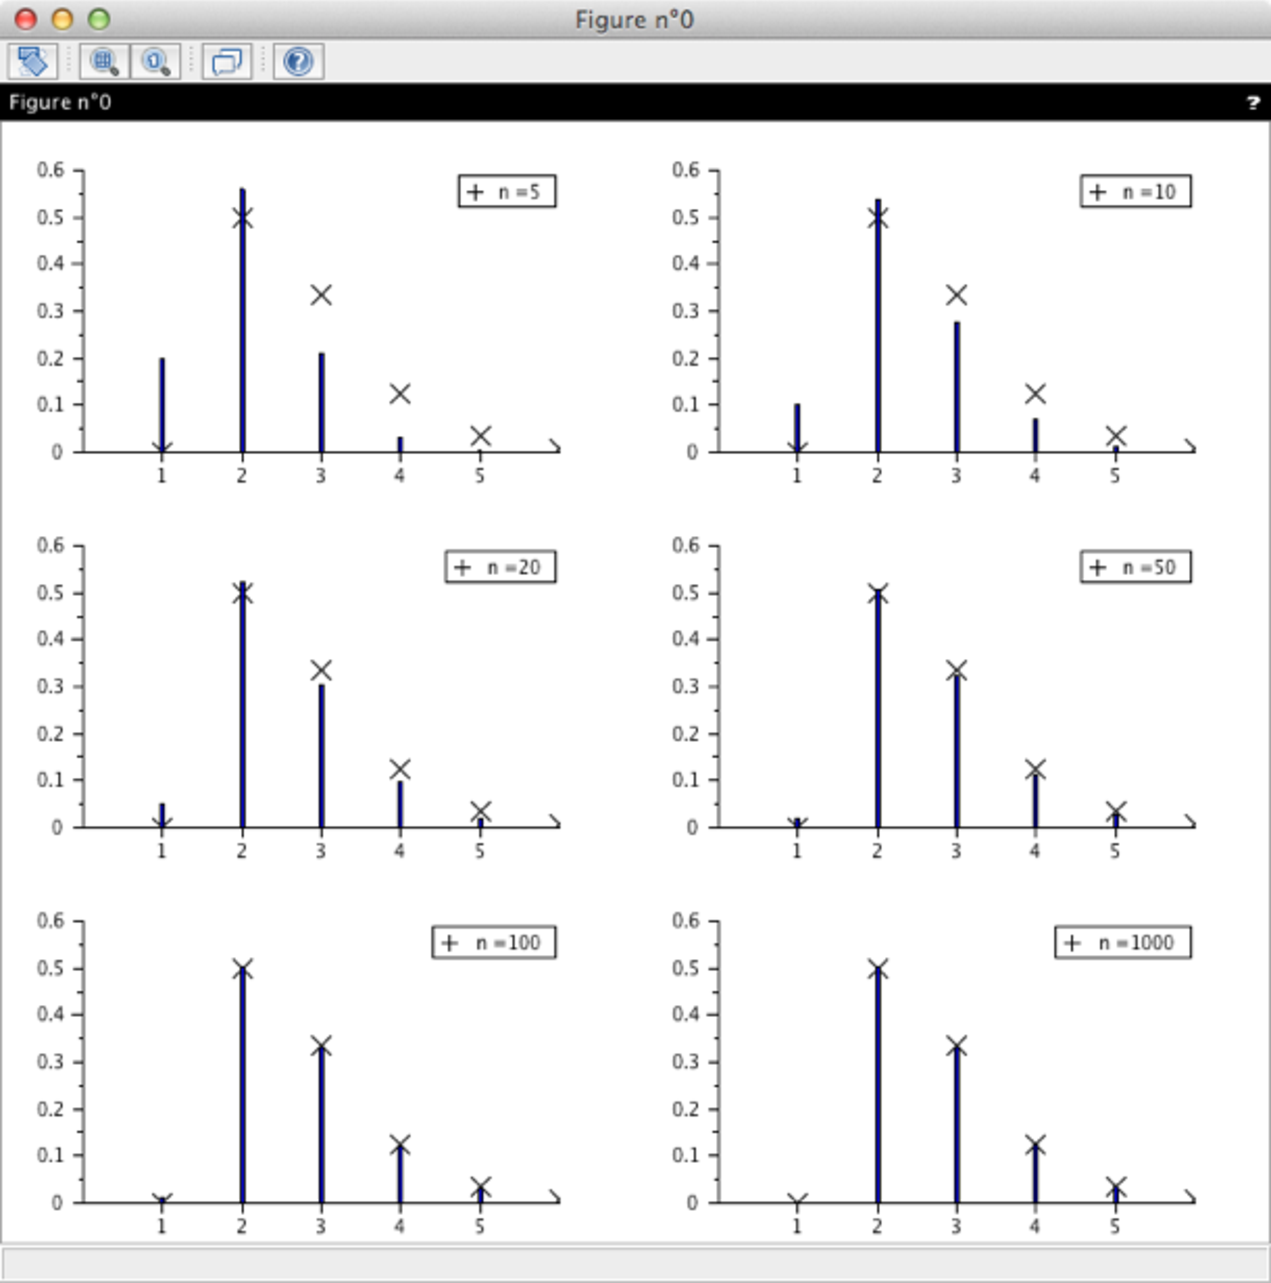
\includegraphics[height=13cm,width=13.13cm]
{Figures/Ecricome_2017/convergence_loi.pdf}
  \end{center}



  \begin{noliste}{a)}
  \item Expliquer ce que représentent les vecteurs renvoyés par les
    fonctions {\tt freqT} et {\tt loitheoY}. \\
    Comment ces vecteurs sont-ils représentés graphiquement dans
    chaque graphique obtenu ?
  
    
    
    
    %\newpage


  \item Expliquer en quoi cette succession de graphiques permet
    d'illustrer le résultat de la question \itbf{13}.
  
        
  \end{noliste}
\end{noliste}


